% !TEX program = tectonic
\documentclass[10pt,a4paper,twocolumn]{article}
\usepackage{iftex}
\ifPDFTeX
  \usepackage[T1]{fontenc}
  \usepackage{lmodern}
  \usepackage[utf8]{inputenc}
\else
  \usepackage{fontspec}        % XeTeX/LuaTeX (tectonic) : UTF-8 natif
\fi
\usepackage[french]{babel}
\frenchsetup{StandardLists=true}
\usepackage[a4paper,margin=1.5cm,columnsep=0.6cm,footskip=0.7cm]{geometry}
\usepackage{amsmath,amssymb}
\usepackage{booktabs}
\usepackage{array}
\usepackage{graphicx}
\usepackage{enumitem}
\setlist[itemize]{leftmargin=1.1em,itemsep=0.5pt,topsep=1.5pt,parsep=0pt}
\setlist[enumerate]{leftmargin=1.5em,itemsep=0.5pt,topsep=1.5pt,parsep=0pt}
\usepackage{xcolor}
\usepackage[font=small,skip=2pt]{caption}
\usepackage{titlesec}
\titlespacing{\section}{0pt}{0.75em}{0.3em}
\titleformat{\section}{\normalsize\bfseries}{\thesection.}{0.4em}{}
\usepackage{hyperref}
\hypersetup{colorlinks=true,linkcolor=blue!50!black,urlcolor=blue!50!black}
\setlength{\parindent}{0pt}
\setlength{\parskip}{0.25em}
\raggedbottom
\setlength{\emergencystretch}{1.5em}
\renewcommand{\topfraction}{0.9}
\renewcommand{\textfraction}{0.05}
\renewcommand{\floatpagefraction}{0.85}
\abovedisplayskip=3pt plus 1pt \belowdisplayskip=3pt plus 1pt
\abovedisplayshortskip=2pt \belowdisplayshortskip=2pt
\newcommand{\code}[1]{\texttt{\small #1}}

\title{\vspace{-1.8em}\textbf{Du corpus brut à la table de backtest : l'entonnoir et les résultats}\\[2pt]
\large Nettoyage backtest 2014--2026 --- fiche de résultats\\[1pt]
\small \code{Nettoyage\_Backtest\_2014\_2026.ipynb} $\to$ \code{transactions\_backtest\_2014\_2026.csv}}
\author{\small Alice Lemaire --- 7 juillet 2026}
\date{\vspace{-2.6em}}

\begin{document}
\maketitle

\section{L'essentiel}
\begin{itemize}
  \item Corpus source-primaire : \textbf{169\,000} transactions uniques (100\,\% de l'index officiel
        House traité, census Sénat documenté).
  \item Entonnoir de nettoyage en \textbf{4 retraits justifiés} $\to$ table de recherche
        \textbf{134\,464 lignes $\times$ 36 colonnes} (\textbf{79{,}6\,\%} conservées).
  \item Validée en externe : \textbf{93{,}5\,\%} (House) / \textbf{92{,}1\,\%} (Sénat) des combinaisons
        de Quiver retrouvées ; \textbf{100\,\%} de senate-stock-watcher ; \textbf{99{,}5\,\%} du mirror
        House 2018--2026.
  \item Tout le doute est \textbf{gardé et flagué} (jamais retiré en silence).
  \item Déjà consommée telle quelle par les notebooks de recherche 05 et 06.
\end{itemize}

\section{L'entonnoir}

\begin{center}
\begin{minipage}{\linewidth}\centering
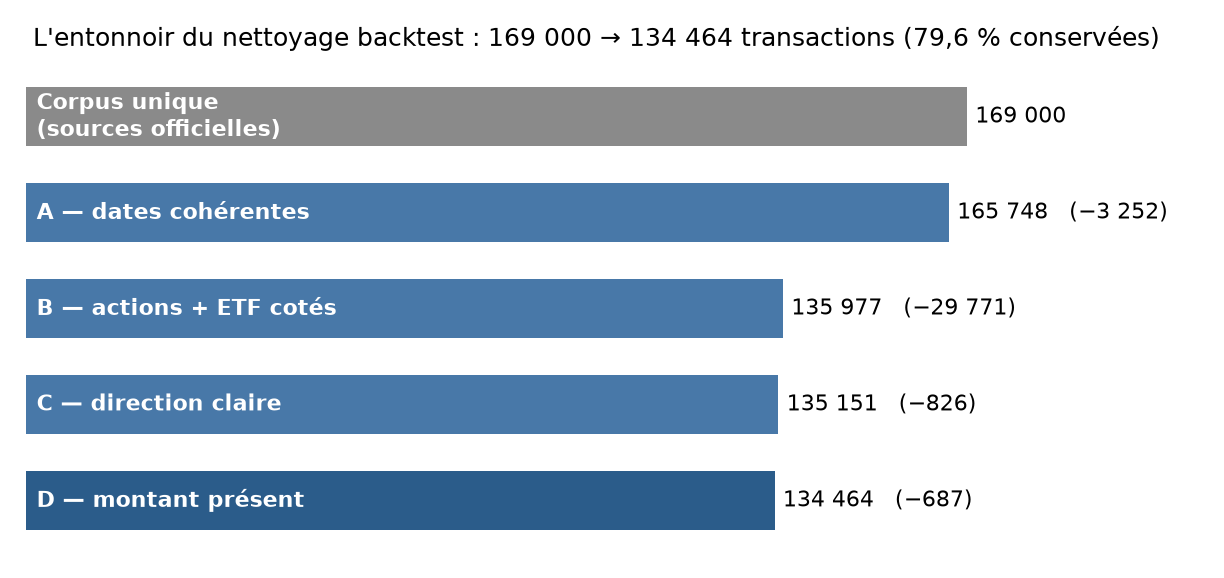
\includegraphics[width=\linewidth]{quality/entonnoir_backtest.png}
\captionof{figure}{Chaque retrait est compté ; aucun autre filtre n'est appliqué.}
\end{minipage}
\end{center}

Les critères, dans l'ordre :
\begin{itemize}
  \item \textbf{A — dates cohérentes} : $\text{lag} = t_{\text{publication}} - t_{\text{transaction}} \ge 0$
        et $2012 \le \text{année} \le \text{année du dépôt}$ (sinon impossible de dater l'entrée) ;
  \item \textbf{B — actions + ETF cotés} : un backtest exige un prix de marché. Retirées : 27\,006 sans
        aucun symbole (munis, obligations, sociétés privées) $+$ 164 malformés (CUSIP, fragments OCR)
        $+$ 2\,601 familles non cotées (options, bons du Trésor) ;
  \item \textbf{C — direction claire} : $\text{direction} \in \{\text{buy},\, \text{sell}\}$
        (les « échanges » n'ont pas de sens directionnel) ;
  \item \textbf{D — montant présent} : $\text{montant} = \frac{lo + hi}{2}$, milieu exact de la
        fourchette STOCK Act.
\end{itemize}

\textbf{Rescue « ticker-first »} : \textbf{21\,878 lignes gardées} dont la case « type d'actif » est
vide mais dont le ticker est une action cotée valide — on décide sur le \emph{ticker}, pas sur la case
déclarée (vide dans 16--31\,\% des cas).

\section{La table finale — aperçu}

\begin{center}
\begin{minipage}{\linewidth}\centering\scriptsize\setlength{\tabcolsep}{2.6pt}
\begin{tabular}{llllrl}
\toprule
\textbf{membre} & \textbf{ticker} & \textbf{sens} & \textbf{transaction} & \textbf{montant \$} & \textbf{secteur}\\
\midrule
Bob Gibbs      & INTC  & buy  & 2014-12-30 & 8\,000{,}5  & Info.\ Tech.\\
Greg Gianforte & BBAVY & sell & 2018-12-12 & 32\,500{,}5 & Cons.\ Staples\\
Kim Dr Schrier & AAPL  & sell & 2021-11-15 & 375\,000{,}5 & Info.\ Tech.\\
Tim Moore      & HOG   & buy  & 2025-12-09 & 32\,500{,}5 & Cons.\ Discr.\\
\bottomrule
\end{tabular}
\captionof{table}{4 lignes réelles (extrait ; 36 colonnes au total, dont \code{disclosure\_date},
parti et commissions \emph{à la date du trade}, \code{etf\_proxy}, flags).}
\end{minipage}
\end{center}

Les 36 colonnes, par famille :
\begin{itemize}
  \item \textbf{identité} : \code{bioguide\_id}, nom, chambre, parti et commissions
        \emph{point-in-time} (résolues à 99{,}1\,\% ; flag « commission clé » : 54{,}6\,\%) ;
  \item \textbf{dates} : transaction, publication, $\text{lag}$ en jours (médiane \textbf{27~j}) ;
  \item \textbf{montant} : milieu exact de fourchette (renseigné à 99{,}4\,\%) ;
  \item \textbf{instrument} : \code{ticker\_yahoo} (renommages appliqués : FB$\to$META\ldots),
        secteur GICS (100\,\% des actions), \code{etf\_proxy} (98{,}8\,\%) ;
  \item \textbf{flags} et \textbf{traçabilité} (document source par ligne).
\end{itemize}

\section{Composition}

\begin{center}
\begin{minipage}{\linewidth}\centering\small\setlength{\tabcolsep}{5pt}
\begin{tabular}{lrr}
\toprule
 & \textbf{n} & \textbf{part}\\
\midrule
House / Sénat          & 122\,814 / 11\,650 & 91{,}3\,\% / 8{,}7\,\%\\
achats / ventes        & 68\,250 / 66\,214  & 50{,}8\,\% / 49{,}2\,\%\\
actions                & 128\,974           & 95{,}9\,\%\\
ETF diversifiés        & 2\,022             & 1{,}5\,\%\\
ETF sectoriels         & 168                & 0{,}1\,\%\\
cotés, classe non résolue (flagués) & 3\,300 & 2{,}5\,\%\\
2014--2019 / 2020--2026 (House) & 56\,706 / 66\,108 & ---\\
\bottomrule
\end{tabular}
\captionof{table}{Composition des 134\,464 transactions.}
\end{minipage}
\end{center}

\begin{center}
\begin{minipage}{\linewidth}\centering
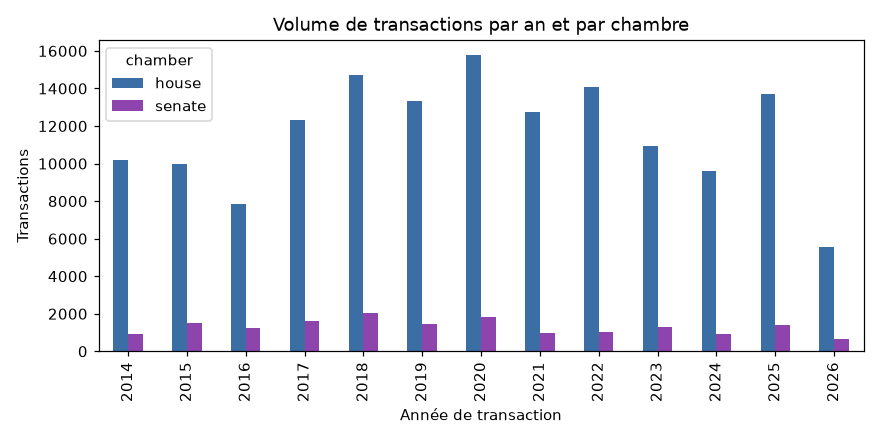
\includegraphics[width=\linewidth]{quality/transactions_par_an.png}
\captionof{figure}{Transactions par année (corpus complet).}
\end{minipage}
\end{center}

\begin{center}
\begin{minipage}{\linewidth}\centering
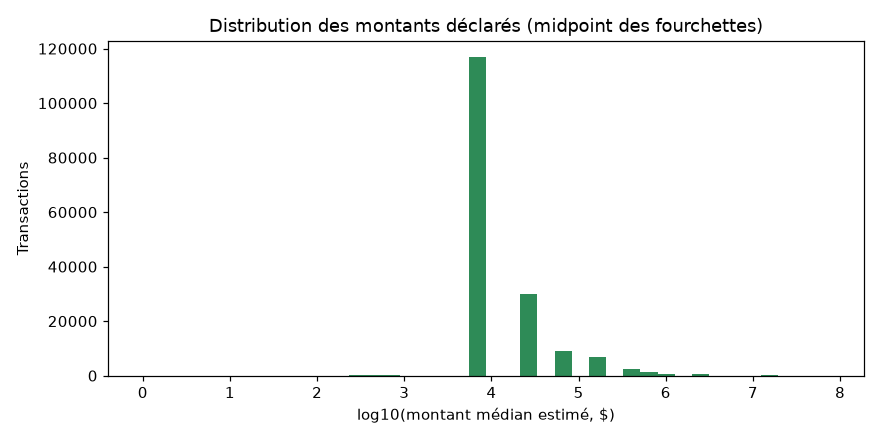
\includegraphics[width=\linewidth]{quality/distribution_montants.png}
\captionof{figure}{Distribution des montants (fourchettes STOCK Act).}
\end{minipage}
\end{center}

\section{Qualité et flags}

\begin{itemize}
  \item Identité rattachée : \textbf{100\,\%} · dates cohérentes : \textbf{99{,}8\,\%} ·
        montants : \textbf{99{,}4\,\%}.
  \item Assertions bloquantes à l'export (bioguide, ticker, montant, direction, chronologie, clé
        naturelle) : le notebook refuse de publier sinon.
\end{itemize}

\begin{center}
\begin{minipage}{\linewidth}\centering\small\setlength{\tabcolsep}{4pt}
\begin{tabular}{lrr}
\toprule
\textbf{doute flagué (jamais retiré)} & \textbf{lignes} & \textbf{part}\\
\midrule
publication $> 45$~j (\code{late\_filing}) & 16\,349 & 12{,}2\,\%\\
publication $> 365$~j                      & 3\,075  & 2{,}3\,\%\\
titre sorti de cote, typé (\code{is\_delisted}) & 3\,542 & 2{,}6\,\%\\
lots multi-comptes (\code{lot\_size} $> 1$) & 11\,873 & 8{,}8\,\%\\
symbole recyclé/fusion (\code{price\_caution}) & 505 & 0{,}4\,\%\\
\bottomrule
\end{tabular}
\captionof{table}{Le doute est signalé, la recherche décide.}
\end{minipage}
\end{center}

\section{Validation externe (résultats)}
\begin{itemize}
  \item \textbf{Quiver Quant} : 93{,}5\,\% / 92{,}1\,\% de ses combinaisons retrouvées ; au trade daté,
        70\,265 + 8\,766 appariés \textbf{au jour exact} ; après enquête, \textbf{31 + 0} combinaisons
        cotées au plus restent inexpliquées. Et on a \textbf{+23\,535 / +2\,951} trades cotés nets
        de plus que lui.
  \item \textbf{senate-stock-watcher} : \textbf{100\,\%} de ses 6\,231 transactions retrouvées.
  \item \textbf{Mirror house-stock-watcher} (mêmes PDF officiels, lecture indépendante) :
        \textbf{99{,}5\,\%} de ses lignes 2018--2026 retrouvées.
\end{itemize}

\section{Limites}
\begin{itemize}
  \item \textbf{582 PTR manuscrits écartés} par décision de périmètre (7{,}1\,\% de l'index,
        concentrés avant 2020) — documentés un par un.
  \item Côté recherche : couverture prix \textbf{87{,}8\,\%} des trades (74\,\% en 2014 $\to$ 99\,\%
        en 2026) $\Rightarrow$ léger biais de survie.
\end{itemize}

\end{document}
